\section{Fensterfunktionen}
Eine wichtige Funktion und ein Hauptfeature der Stream Analytics-Abfragesprache SAQL bzw. von Azure Stream Analytics ist die Möglichkeit, mit Zeitfenstern zu arbeiten. Anwendbare Fensterfunktionen sind [6]:
\begin{itemize}
\item Azure-Blobspeicher 
\item TumblingWindow
\item HoppingWindow
\item SlidingWindow
\end{itemize}
Diese Funktionen erlauben es für Streamingdaten temporale Vorgänge durchzuführen. Die Ausgabe eines Fensters ist ein einzelnes Ergebnis, welches auf der verwendeten Aggregatfunktion basiert. Dieses Ergebnis besitzt dann einen Zeitstempel vom Ende des Fensters, die immer eine fest definierte Länge besitzen. Alle angewandten Fensterfunktionen bzw. deren Ergebnisse sollten schließlich noch mit einer GROUP BY-Klausel entsprechend zusammengeführt werden [7]. 
Beispielsweise soll nun eine Abfrage gestartet werden. Diese Aggregatfunktion soll aufzeigen, wie viele Autos einer speziellen Farbe alle fünf Minuten eine Mautstelle passieren [6]. Mit TumblingWindow wird ein Datenstrom in einzelne Zeitsegmente unterteilt. Für diese unterteilten Segmente wird dann eine Funktion ausgeführt. Die eben beschriebene Abfrage kann hier 1:1 implementiert werden. Bei den rollierenden Fenstern gibt es keine Überlappungen und ein Ergebnis kann nicht zu mehreren Fenstern gehören. Bei HoppingWindow wird immer für einen festen Zeitraum einen Sprung nach vorne durchgeführt. Grundsätzlich kann dieser Ansatz wie das TumblingWindow angesehen werden, bloß überlappen sich die sich wiederholenden Fenster. Durch diesen Umstand kann es sein, dass ein Ergebnis zu mehreren Fenstern gehören kann. Die Abfragen lässt sich hier ähnlich ausdrücken, allerdings kann hier unabhängig von der Fenstergröße eine Ausgabe erzeugt werden. Es könnte hier beispielsweise einmal pro Minute ausgegeben werden, wie viele Autos einer speziellen Farbe alle fünf Minuten diese Mautstelle anfahren. SlidingWindow hingegen erzeugt nur ein Ereignis, wenn entsprechende Anforderungen erfüllt sind bzw. Ereignisse auftreten [7]. Auch hier können Ergebnisse zu mehreren Fenstern gehören. Dieser Ansatz lässt die Abfrage zu, in welchen 5-Minuten-Zeitfenstern zehn oder mehr Autos einer speziellen Farbe die Mautstelle erreichen. SlidingWindow ist somit für den Umgang mit relativ spärlichen Ergebnismengen geeignet. Diese Konzepte sind in Abbildung 3 dargestellt [6].
\\ \\

\begin{figure}[h!]
	\centering
	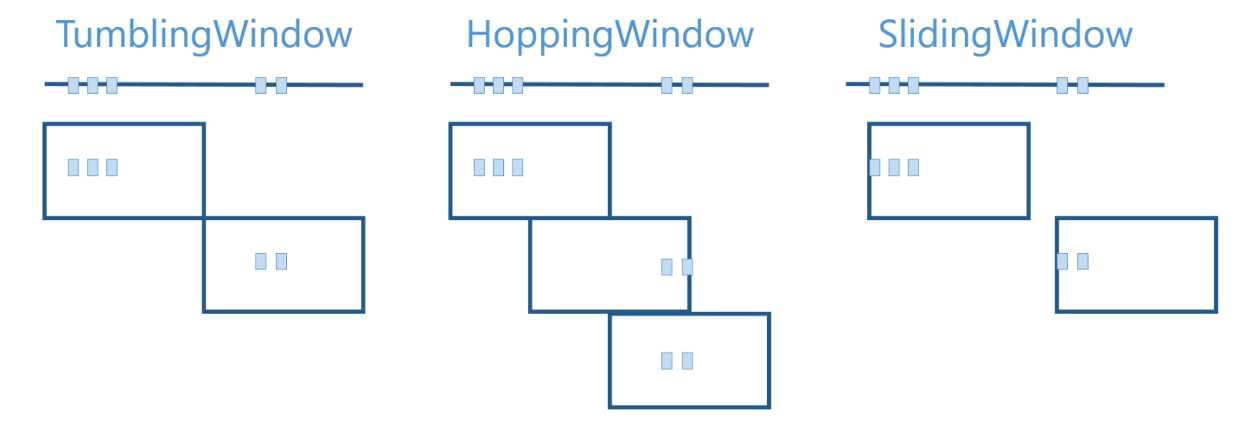
\includegraphics[width=1.0\linewidth]{images/fensterfunktionen}
	\caption{Fensterkonzepte} %Generelle
	\label{fig:window_concepts}
\end{figure}
